\documentclass[11pt,letterpaper]{article}
%\documentclass[11pt,a4paper]{report}

\usepackage{amssymb,amsmath,amsthm} 
\usepackage[margin=2cm]{geometry}
\usepackage{fancyhdr}
\usepackage{enumitem}
\usepackage[compact]{titlesec}
\usepackage{graphicx,ctable,booktabs,subcaption}

\usepackage{xparse,hyperref,parskip}

%\newcommand{\abs}[1]{\left|#1\right|}

\newcommand{\semester}{Spring 2022}
\newcommand{\due}{Thursday, April 28}


\pagestyle{fancy}
\lhead{ }
\chead{\footnotesize Math 3338\quad  Numerical Methods\quad  \semester}
\rhead{\footnotesize \thepage}
\setlength{\parindent}{0cm}
\setlist{noitemsep}



\newcommand{\D}{\text{d}}

\newtheorem{theorem}{Theorem}

\input{defs.tex}

%Defines the problem environment with arguments Points and Solution gap
\input{problem_env.tex}



\begin{document}

\begin{center}
{\huge{\bf  Numerical Methods}} \\[1.5ex]
{\bf Math 3338 -- \semester}\\[1.5ex]
{\Large{\bf Worksheet 28\ \\[2ex] Logistic Regression}}\\
\end{center}
\vspace{2mm}


\section{Reading}

\begin{table}[!ht]
 \centering
 \begin{tabular}{lc}
   CP & - \\
 NMEP &  -
 \end{tabular}
\caption{Sections Covered}
\end{table}

Consider the graph in Figure \ref{fig:classification}.
\begin{figure}[!h]
 \centering
 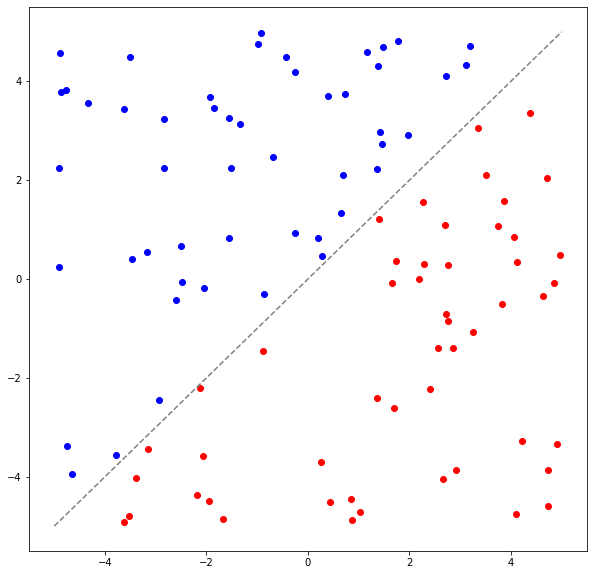
\includegraphics[width=.4\textwidth]{images/classification.png}
 \caption{A basic classification problem.}
 \label{fig:classification}
\end{figure}
You want to create a condition to separate the red and blue dots\footnote{Let's hope I didn't print this in black and white.}. In this case the condition is the dots are red if $x>y$ and blue otherwise, it's a very simple condition. I put the line $y=x$ dashed to emphasize the boundary. However, if this is a much higher dimensional problem it becomes far more difficult. This is where \emph{logistic regression} is useful. 

Logistic regression is used to classify items that in two states, or binary problems. In this case we'll say the blue dots correspond it 1 and red is 0. So if we are given the point $(5,2)$ that is 0 since $x>y$ and $(2,8)$ is 1 since $x\le y$. We are going to build a logistic regression model to separate these points. 

Here is the big idea. We are going to create a function $F$ that takes a point $x$ (in our case $x=[x_1,x_2]$ since we have two coordinates) and outputs a number between 0 and 1. If $F(x)\ge .5$ then we'll say that $x$ is a 1 and vice-versa. The easiest way to understand this is to build it in reverse. First we want a function that always returns a value between 0 and 1 and doesn't faff about. 
The answer is the sigmoid function as seen in Figure \ref{fig:sigmoid_graph}.
\begin{figure}[!h]
 \centering
 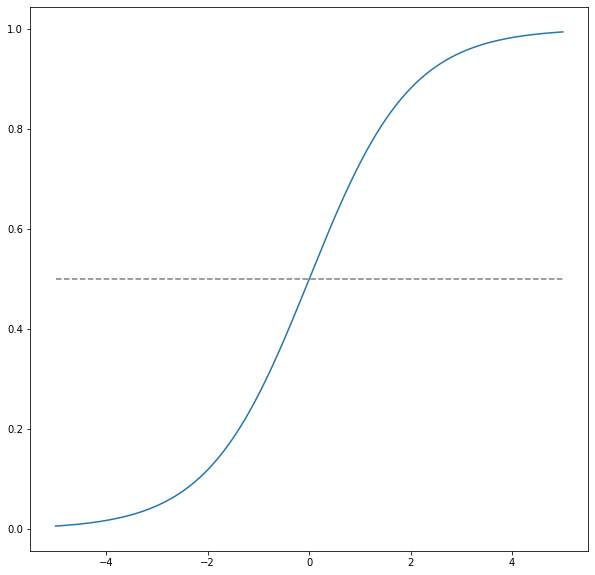
\includegraphics[width=.4\textwidth]{images/sigmoid_graph.png}
 \caption{The sigmoid function.}
 \label{fig:sigmoid_graph}
\end{figure}
The equation of this graph is 
\begin{equation}
\label{eqn:sigmoid}
\sigma(x) = \frac{1}{1+e^{-x}}
\end{equation}
Notice this function spends very little time between 0 and 1, that makes it ideal as a final step\footnote{$\tanh$ is another good option}, it separates values effectively. 

What do we put into the sigmoid? A weighted sum of the inputs. In our case that means something of the form $w_1x_1+w_2x_2 + b$. What is the $b$? It's a bias term that helps correct the weighted sum, it tends to be useful. You probably recognized this as an offset plane, that's right it's essentially linear regression. How do we actually find the correct weights and bias? Optimization. 

Let's start by saying $w_1 = w_2 = b = 1$ with an input of $x=[2,1]$. We know $y=0$ (this is the true output), let's make a prediction based on our current weights. 
\begin{align*}
 \hat{y} = & \sigma(1\cdot 2 + 1\cdot 1 + 1) \\
         = & \sigma(4) \\
         = & 0.9820137900379085
\end{align*}
This is wrong, we really wanted $\hat{y}\sim 0$. We need a function that will tell us how wrong we are. That turns out to be something called \emph{binary crossentropy}. 
\begin{equation}
 \label{eqn:binary_crossentropy}
 \mathcal{L}(\hat{y},y) = -y\ln(\hat{y}) - (1-y)\ln(1-\hat{y})
\end{equation}
Let's compute this for our previous prediction,
\begin{align*}
\mathcal{L}(0.9820137900379085,0) = & -0\ln(0.9820137900379085) - (1-0)\ln(1-0.9820137900379085)\\
 = & 4.01814992791781
\end{align*}
This is fairly large. You should stop and think about why this is the ``right'' thing to use. Think about the possible values of $y$ and what will happen when $y\sim \hat{y}$. 

We want to minimize $\mathcal{L}(\hat{y},y)$. We've done this in the past and we'll use gradient descent. Our variables are $w$ and $b$, but it will be useful to have a couple of temporary variables as well $z = w\cdot x + b$ and $a = \sigma(z)$. The variable $a$ isn't really useful right now, but it will be next time. 


There is one final note to make before we start doing some real math. The standard notation. We will, by default, be caring about $\frac{d\mathcal{L}}{dv}$ where $v$ is some variable. This tends to be quite a bit to type into computes and gets cumbersome. We will abbreviate $\frac{d\mathcal{L}}{dv}$ as just $\D v$. As a mathematician, this kinda hurts. But it does make some things nice. 

We want to perform gradient descent on $w$ and $b$. That means we will be updating $w=w-\alpha \D{w}$ and $b = b - \alpha \D b$, so we need to find $\D w$ and $\D b$. This just the chain rule,
\begin{align*}
 \D w = & \frac{d\mathcal{L}}{dw} & \D b = &  \frac{d\mathcal{L}}{db} \\
 = & \D z\frac{dz}{dw} &  = & \D z\frac{dz}{db} \\
 = & \D z * x &  = & \D z \\
\end{align*}
The $*$ is coordinate wise multiplication. Of course, now we need to find $\D z$. 
\begin{align*}
 \D z = & \frac{d\mathcal{L}}{dz} \\
     = & \frac{d\mathcal{L}}{d\sigma} \frac{d\sigma}{dz}\\
     = & \left(\frac{-y}{\sigma(z)} + \frac{(1-y)}{1-\sigma(z)}\right)\sigma(z)(1-\sigma(z)) \\
     = & \sigma(z) - y
\end{align*}
Notice, $\D z$ is kinda $\hat{y}-y$, which it really should be. 


We're almost done, but we've only done this for a single sample. In reality we'll have a lot\footnote{Potentially millions} of samples. We need to generalize and make it vectorized. The main difference should be capital letters vs lower case. 
\begin{align*}
 X = & \begin{bmatrix}
   x^1_1 & x^2_2 & \dots & x^m_1\\
   x^1_2 & x^2_2 & \dots & x^m_2
 \end{bmatrix}
 & W = & [w_1, w_2] & & \vec{b} = [b]
\end{align*}
The samples in $X$ are arranged in columns, so there are $m$ samples each with $2$ observations. $W$ is a row vector with $2$ columns, which matches the number of observations. $\vec{b}$ is a vector with a single column, which matches the number of rows in $W$. Using these, 
\begin{equation*}
 Z = W^TX+\vec{b}
\end{equation*}
that is a transpose on $W$. This is a vectorized operation, so $W^T$ and $\vec{b}$ are being broadcast to the correct shapes. The loss function is just a summation,
\begin{equation*}
 \mathcal{L}(\hat{y},y) = \sum_{i=1}^m \mathcal{L}(\hat{y}_i,y_i)
\end{equation*}
I abused notation here slightly by using $\mathcal{L}$ twice to mean different things. But oh well. Finally,
\begin{align*}
\D Z = & \sigma(z) - y & \D W = & \frac{1}{m}dZ\cdot X^T & \D b = & \frac{1}{m}\sum dZ
\end{align*}
The $\frac{1}{m}$ act as regularization to prevent the summations from blowing up. 



\newpage

\begin{center}
{\huge{\bf  Numerical Methods}} \\[1.5ex]
{\bf Math 3338 -- \semester}\\[1.5ex]
{\Large{\bf Homework 28 (Due: \due)}}\\
\end{center}
\vspace{2mm}

\begin{problem}
 Verify the derivatives in $\D z$. 
\end{problem}



\begin{problem}
 Make a function called \texttt{logistic\_regression(X,y,alpha=.1,N=100)} that implements logistic regression and does \texttt{N} iterations. Initialize the weights randomly using \texttt{numpy.random.randn} and make them small by multiplying by .01. Return the weights and bias term.
 
 Also make a function called \texttt{predict(X,W,b)} that makes predictions based on the weights and bias.
\end{problem}

\begin{problem}
\label{3}
 The file ``hw\_28-data\_01.pickle'' contains a pair $[X,y]$ and the file ``hw\_28-predict\_01.pickle contains an $\hat{X}$.
 \begin{enumerate}
  \item Apply logistic regression.
  \item Plot this data using two different colors for $X$ based on their $y$ value. Add the boundary line given by the weights and bias to you graph. Remember, we have $w_1x+w_2y +b = 0$. You can solve for $y$ to find the boundary. You should use a subplot with 2 rows (you'll be adding another graph to it).
  \item Use your model to make predictions based on $\hat{X}$.
  \item Plot the $\hat{X}$ data using two different colors based on their $\hat{y}$ predictions. Does your data fit your predicted boundary?
 \end{enumerate}
\end{problem}




\begin{problem}
\label{4}
 The file ``hw\_28-data\_02.pickle'' contains a pair $[X,y]$ and the file ``hw\_28-predict\_02.pickle contains an $\hat{X}$.
 \begin{enumerate}
  \item Apply logistic regression.
  \item Plot this data using two different colors for $X$ based on their $y$ value. Add the boundary line given by the weights and bias to you graph. Remember, we have $w_1x+w_2y +b = 0$. You can solve for $y$ to find the boundary. You should use a subplot with 2 rows (you'll be adding another graph to it).
  \item Use your model to make predictions based on $\hat{X}$.
  \item Plot the $\hat{X}$ data using two different colors based on their $\hat{y}$ predictions. Does your data fit your predicted boundary?
 \end{enumerate}
\end{problem}



\begin{problem}
 You should have noticed that the boundary for Problem \ref{3} was pretty good, but Problem \ref{4} was awful. Why did this happen? Further, why was the boundary for the predictions perfect?
\end{problem}

\end{document}




































